\documentclass[12pt]{article}
\usepackage[utf8]{inputenc}
\usepackage{MnSymbol}%
\usepackage{wasysym}%
\usepackage{amsfonts}
\usepackage{graphicx}
\usepackage{grffile}
\usepackage{amsmath}
\usepackage{csquotes}
\usepackage{listings}
\usepackage{subcaption}
\usepackage{wrapfig}
\usepackage{esvect}
\usepackage[section]{placeins}
\usepackage{minted}
\graphicspath{ {/Users/anthonymaylath/Documents/NYU/High_Performance_Computing/HW/HW1/} }
\DeclareGraphicsExtensions{.pdf,.png,.jpg}

\batchmode

\title{High Performance Computing - HW 6}
\author{Anthony Maylath}

\lstset{
numbers=left, 
numberstyle=\small, 
numbersep=8pt, 
frame = single, 
language=Pascal, 
framexleftmargin=15pt}

\begin{document}

\maketitle

\begin{center}

The Courant Institute for Mathematical Sciences, New York University \\ 

\end{center}

\DeclareGraphicsExtensions{.pdf,.png,.jpg}

\setcounter{MaxMatrixCols}{13}

\section{Excersise 1}

\subsection{Introduction: Pricing Exotic Financial Derivatives}

Consider a financial derivative whose payoff depends on several assets. Say the product also provides an option for the holder. A popular example of such a product would be a `''Worst of Option'' which has pay off:

\begin{align}
P(S_T) = max\Big(\min_{s_T \in S_T}(S_T) - K,0\Big) 
\end{algin}

where $S_T$ is a set of assets and time $T$ represents the experation of the product. Obtaining a reasonable price for such assets is not tractable analytically. Financial Engineers typically deploy Monte Carlo simulations to evaluate such products. Typically, the approch would involve simulating a stochastic differential equation of the form:

\begin{align}
ds_{i,t} = a(s_{i,t},t)dt + b(s_{i,t},t)dW_t
\label{eq2}
\end{align}

where $s_{i,t}$ is the price of asset $i$ at time $t$ and $W_{t}$ is a Brownian Motion, possibly correlated with the other assets which determine the  payoff.

\subsection{Multi-Variable Monte Carlo}

A reasonable way to solve \ref{eq2} would be to discretize each $s_{i,t}$ into time steps and model $dW_{t}$ with draws from a random normal. For instance, the Milstein scheme is a popular discretation \cite{glasserman}. To achive quadratic convergence with the Milstein scheme, we typically need the time step to be proportional to the square of the space step, which can result in a dense grid.\\

A standard method to improve cost leverages the linearity of expectation, $E[p_1] = E[p_0] + E[p_1-p_0]$, where $p_1$ is the price of our complex derivative and $p_0$ is the price of a simple derivative highly correlated to $p_1$. Since $p_0$ is simple, we do not need a dense grid to estimate it. Likewise, we can allow a sparse grid as $p_1 - p_0$ is small relative to $p_0$. The approch is known as a control variate.\\

Even with the improvement, the complexity of exotic derivatives generally require a dense grid to acheve reasonable convergence to he expectation. Such a grid can require heavy computing resources to evaluate in a fast pace trading enviornment.\\

Michael Giles et al. \cite{giles} have propsed an extension to the standard control variate which uses several control variates:

\begin{align}
E[p_L] = E[p_0] + \sum_{l=1}^LE[p_l - p_{l-1}]
\end{align}

To evaluate an exotic derivative in the single control variable case, evaluate a portfolio of vanilla derivatives with similar behavior to the exotic product for little cost using analytical methods. The portfolio of vanillas are deployed as the control variate. We could then assign each path of the evauation to a seperate processor to solve the problem with high computing resources.\\

Say we want to evaluate the exotic derivative at more than one point over the input space. For the inner valuations of the inputs, we could use the neighboring points as control variates. The approch is called Multi-Level Monte Carle (MLMC). However, when we use neighboring paths in the valuation, we can no longer dispatch our valuations to run on seperate processors independantly. As a resolution, message passing software could be leveraged to comunicate control variates from neighboring points in the grid.\\

 The method starts with evaluations on a fine grid and gradually moves to a course grid as more control variates are added. The result tends to be many evaulations on a course grid, with only a few evaluations on a fine grid. Load balancing can be tricky in such a situation as the overhead of scheduling can cost more than the benefit from parallelization for small jobs. Scheduling can become so complex that it may consume more developer time than writing the code to evaluate the expectation \cite{gmeiner}.

\subsection{Implementation on High Performance Machines}

Gmeiner, Drzisgn, et al. \cite{gmeiner} explore the performance of MLMC with multigrid strategies on supercomputing resources. The paper applies the MLMC to uncertainty quantification for solutions to 3D partial differential equations. The problem is a bit different than the evaulation of financial derivatives, but the paper provides detailed performance results useful enough to understand how the method could perform on other applications.\\

The paper deploys the peta-scale German supercomputer, JUQUEEN, which features 28,672 nodes with 16 GB memory and 16 1.6 Ghz cores. As of November, 2017, JUQUEEN was ranked 22 on the supercomputer top 500 list. For a grid of $1.1*10^9$ mesh nodes and three levels, the authors found the time to resolve each of the levels was between two and three minutes with static scheduling. WIth the addition of each control variate the compute time went up by a few seconds.\\

As the number of computing resources increased, the authors found the computation time declined at a sub-linear rate. The marginal gain declined as overhead from load balancing small tasks began to outweigh the benefit of more processors. The paper deployed between 2,048 and 131,072 processors to obtain the results.

\section{Exercise 2}

I make the following changes lines 54 and 55 in \textit{MMult0.ccp} to track the flop rate and bandwidth:

\begin{lstlisting}[language=C++,frame=none]
double flops = NREPEATS*m*n*k*10/1e9/time;
double bandwidth = NREPEATS*m*n*k*sizeof(double)/1e9/time;
\end{lstlisting}

where the factor of 10 occurs in the flop rate as we perform 10 flops in the inner most loop of function \textit{MMult0()}. For the bandwidth, I only count the write to array on line 24. I ran the program with a 2 core 2.4 GHz Intel Core i5 and 8 GB of DDR3-1600 memory.\\

Figures \ref{O0opt} and \ref{O3opt} show the time in seconds, flops, and bandwidth against the dimension for -O0 and -O3 optimizations. Notice the secondary axis for the -O0 optimization. For both -O0 and -O3 optimizations the compute time went up significantly with the matrix dimension. The performance of the -O0 optimization was much worse, taking as much as 77 seconds to evaluate dimension 580. The flop rate and bandwidth also seem to be much better with the -O3 optimzation with as much as 9.7 Gflop/s compared to just over 1 Gflop/s with -O0. The results also show a jump in Gflop/s and bandwidth after the first run on -O3. It would be interesting to see if the compiler somehow memorizes the data after the first run.

\begin{figure}
  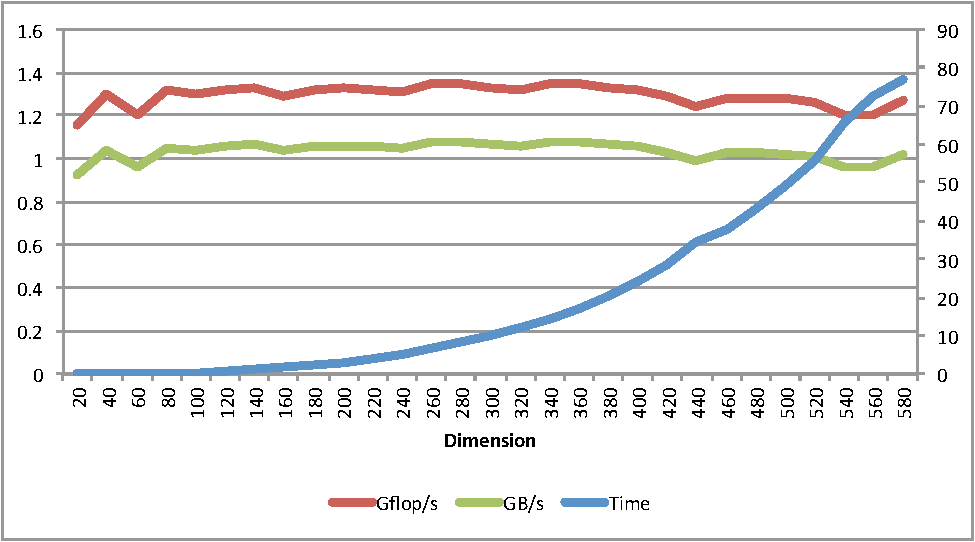
\includegraphics[width=\linewidth]{HW1_Q2_O0.pdf}
  \caption{-O0 Compiler Optimization}
  \label{O0opt}
\end{figure}

\begin{figure}
  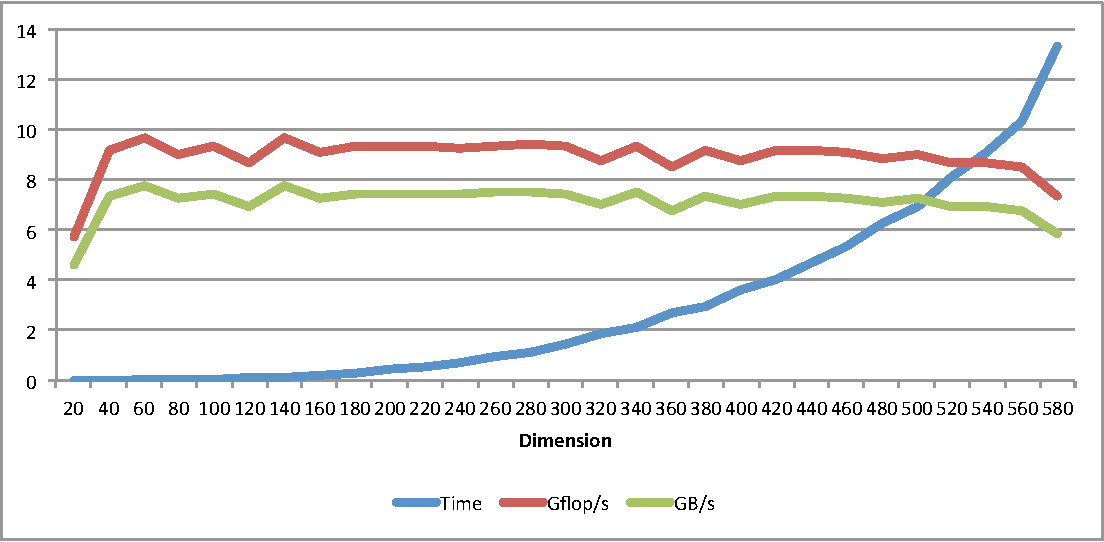
\includegraphics[width=\linewidth]{HW1_Q2_O3.pdf}
  \caption{-O3 Compiler Optimization}
  \label{O3opt}
\end{figure}

\section{Exercise 3}

\subsection{Parts (a),(b)}

The attached c program, \textit{laplace\_dyn.c}, solves the one dimensional Laplace equation for a given dimension. The first, second, and third command line arguments specify the dimension, max iterations, and solver. The user can choose between Jacobi and Gauss-Seidel for the solver. The program terminates when either the maximum iteration has been reached or when the initial error is reduced by a factor or $10^6$. Note that I import the file ``utils.h'' to time my code. As a result, a c++ compiler will be needed. My code listing for Exercise 3 can be found in the Appendix.

\newpage

\subsection{Part (c)}

Table \ref{compIter} pesents the number of iterations to convergence for varying solvers and dimensions. For $N=100$, the program stops when the error reduces by $10^6$. However, for $N=10,000$ we make the threshold smaller as the size of the system requires significant compute power to solve. Gauss-Seidel seems to perform about twice as good for different $N$ compared to Jacobi.\\

\begin{table}[h!]
\centering
\begin{tabular}{ |c|c|c| }
\hline
 Solver & N & Iterations \\ 
 \hline
Jacobi & 100 & 33,107\\ 
Jacobi &  10,000 & 87 \\ 
GS & 100 & 16,555 \\ 
GS &  10,000 & 44 \\ 
 \hline
\end{tabular}
 \caption{Number of Iterations to Converge}
 \label{compIter}
 \end{table}

Table \ref{compTime} shows the run time for different compiler optimizations, solvers, and dimensions. Table \ref{compTime} also assumes a max iteration of 100 for the solver. The -O3 optimization tends to perform about twice as good as -0O.

\begin{table}[h!]
\centering
\begin{tabular}{ |c|c|c|c| }
\hline
 Compiler & Solver & N & Time \\ 
 \hline
 -O0 & Jacobi & 100 & 0.00767\\ 
 -O0 & Jacobi &  10,000 & 63.94689 \\ 
 -O0 & GS & 100 & 0.007544 \\ 
 -O0 & GS &  10,000 & 63.87483 \\ 
 -O3 & Jacobi & 100 & 0.002311 \\ 
 -O3 & Jacobi &  10,000 & 23.744126\\ 
 -O3 & GS & 100 & 0.001867 \\ 
 -O3 & GS &  10,000 & 23.773413\\ 
 \hline
\end{tabular}
 \caption{Timings for Max Iterations = 100}
 \label{compTime}
 \end{table}



\newpage

\begin{thebibliography}{999}

\bibitem{glasserman}
  Paul Glasserman,
  \emph{Monte Carlo Methods in Financial Engineering}.
  Springer Science + Business Media, Inc. 233 Spring Street, New York, NY 10013 USA,
  2003.
  
\bibitem{giles}
  Michael B. Giles,
  \emph{Multilevel Monte Carlo Path Simulation}.
  Operations Research, Vol. 56, No. 3, May-June 2008, pp. 607-617.
  
\bibitem{gmeiner}
Bjorn Gmeiner, Dainel Drzisgn, Ulrich Rude, and Robert Scheichl,
  \emph{Scheduling Massively Parallel Multigrid for Multilevel Monte Carlo Methods}.
  SIAM Journal on Scientific Computing, July 2016.

\end{thebibliography}

\newpage

\section{Appendix: Code Listing for Question 3}

\subsection{Utility Functions}

\begin{minted}[%
 breaklines]{C}
//Helper functions for HW1 Question3
//Anthony Maylath 2/2/2019

//Function to initialize A matrix and f array
void iniLaplace(double *f, double **A, double *u, double h, int N){
	for(int i = 0; i<N; i++){
		//Initialize function and starting guess
		f[i] = 1.0; u[i] = 0.0;
		
		//Initialize second derivative matrix
		for(int j = 0; j<N; j++){
			if(i == j){A[i][j]=2.0/h/h;}
			else if(i == j-1){A[i][j]=-1.0/h/h;}
			else if(i == j+1){A[i][j]=-1.0/h/h;}
			else {A[i][j]=0;}
		}
	}
}

//Run one iteration of Jacobi method
void jacobi(double *f, double **A, double *u, int N){
	
	double sp = 0;
	double *tp = (double *)malloc(N*sizeof(double));
	for(int i = 0; i<N; i++) tp[i] = 0.0;

	for(int i = 0; i<N; i++){
		//Compute sumproduct for each i
		sp = 0;
		for(int j = 0; j<N; j++){
			if(i != j){sp += A[i][j]*u[j];}
		}

		//Compute new iteration
		tp[i] = (f[i] - sp)/A[i][i];
	}

	//Copy tp into u and free tp
	for(int i = 0; i<N; i++) u[i] = tp[i];
	free(tp);
}

//Run one iteration of Gauess-Seidel
void solveGS(double *f, double **A, double *u, int N){
	double sp = 0;

	for(int i = 0; i<N; i++){
		//Compute sumproduct for each i
		sp = 0;
		for(int j = 0; j<N; j++){
			if(i != j){sp += A[i][j]*u[j];}
		}

		//Compute new iteration
		u[i] = (f[i] - sp)/A[i][i];
	}
}

/*Vector matrix multiplication
Multiply matrix A and vector u;
store the result in b*/
void AuMult(double **A, double *u, double *b, int N){
	for(int i = 0; i<N; i++){
		b[i] = 0;
		for(int j = 0; j<N; j++)
			b[i] += u[j]*A[i][j];
	}
}

/*Vector subtracttion
Subtract vector f from u and store the result in b*/
void vecSub(double *u, double *f, double *b, int N){
	for(int i = 0; i<N; i++){
		b[i] = u[i] - f[i];
	}
}

/*Compute 2 norm of a vector b*/
double norm2(double *b, int N){
	double res = 0.0;
	for(int i = 0; i<N; i++)
		res += b[i]*b[i];
	return sqrt(res);
}

/*Compute error between Au and f*/
double error2(double **A, double *u, double *f, int N){
	double *temp = (double *)malloc(N*sizeof(double));
	double res;

	//Compute Au
	AuMult(A,u,temp,N);
	//Compute Au - f
	vecSub(temp,f,temp,N);
	//Return 2norm
	res = norm2(temp, N);
	//Free memory
	free(temp);

	return res;
}
\end{minted}

\subsection{Main Engine}

\begin{minted}[%
 breaklines]{C}
/*Anthony Maylath C code to solve 1D Laplace*/
#include <stdio.h>
#include <stdlib.h> 
#include <math.h>
#include <string.h>
#include "hw1q3_utils.h"
#include "utils.h"

//Function declarations
void iniLaplace(double *f, double **A, double *u, double h, int N);
void jacobi(double *f, double **A, double *u, int N);
void AuMult(double **A, double *u, double *b, int N);
void vecSub(double *u, double *f, double *b, int N);
double norm2(double *b, int N);
double error2(double **A, double *u, double *f, int N);

int main(int argc, char* argv[]){
	/*Iterative solving for linear systems
	argv[1]: represents dimension of matrix (int)
	argv[2]: mac number of iterations (int)
	argv[3]: represents type of solver. "jacobi" or "GS" (string) 
	default solver is Gauss-Seidel*/
	int N = atoi(argv[1]);
	int num_iter = atoi(argv[2]);

	//Allocate space for arrays
	double *f = (double *)malloc(N*sizeof(double));
	double *u = (double *)malloc(N*sizeof(double));
	double **A = (double **)malloc(N*sizeof(double));
	//Allocate second dimension
	for(int i = 0; i<N; i++)
		A[i] = (double *)malloc(N*sizeof(double));
	
	//Declare solver to use for computation
	void (*solver)(double *f, double **A, double *u, int N);
	solver = !strcmp("GS",argv[3]) ? solveGS : jacobi;

	printf("Starting %s solver with %d Dimensions and "
		 "%d max iterations\n",argv[3],N,num_iter);

	double err0, err=10000, h = 1.0/N, tol = 1e6;

	//Initalize problem statement
	iniLaplace(f,A,u,h,N);
	
	//Initial error
	err0 = error2(A,u,f,N);
	printf("Initial error is: %f\n",err0);

	Timer t;
    t.tic(); //Start timer
	int i = 0;
	while((i<num_iter) && (err0/err < tol)){
		solver(f,A,u,N);
		err = error2(A,u,f,N);
		//Print error for every 100 iterations
		if(i%100==0)
		 	printf("Error for iteration %d is %f\n", i, err);
		i++;
	}

	// for(int i = 0; i<N; i++)
	//  	printf("Entry %d is %f\n", i, u[i]);

	//Time results
	printf("Run time: %f\n Number of Iterations : %d\n", t.toc(),i);

	//Free malloced memory
	free(f); free(u);
	for(int i = 0; i<N; i++)
		free(A[i]);

}
\end{minted}

\end{document}